\section{Durchführung}
\label{sec:Durchführung}
Der Versuch wird wie in der Abbildung \ref{fig:Aufbau} aufgebaut.
\begin{figure}
    \centering
    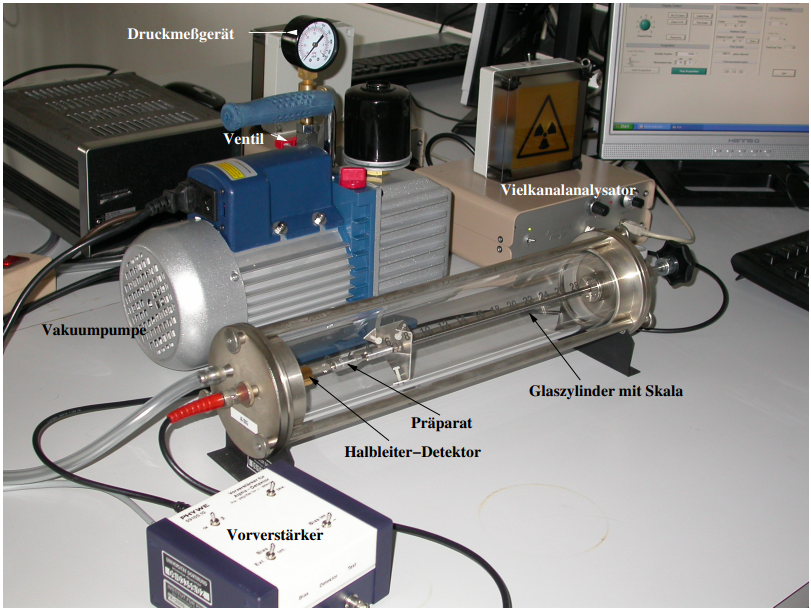
\includegraphics[scale=0.5]{content/Aufbau 701.png}
    \caption{Versuchsaufbau.}
    \label{fig:Aufbau}
\end{figure}
Bei dem Präparat handelt es sich um ein Am-Präparat. Der Vielkanalanalysator ist mit dem Computer verbunden.
Zu Beginn wird im Programm MCA wird der Schalter auf connectet gestellt sowie der Vorverstärker und der Vielkanalanalysator werden eingeschaltet.\\


\subsection{Bestimmung der Reichweite von alpha-Strahlung}

\noindent Zur Messung der Reichweite und des Energieverlust der $\alpha$-Strahlung wird die Messzeit im Programm auf $\qty{120}{s}$ gestellt.
Es wird der erste Abstand zwichen dem Halbleiter-Detektor und dem Am-Präparat über die Feststellschraube am Glaszylinder eingestellt.
Das rote Ventil wird geöffnet und die Vakkumpumpe wird angestellt. 
Wenn das Druckmessgerät $\qty{0}{mbar}$ anzeigt, wird das Ventil wieder geschlossen und die Pumpe ausgestellt.
Im Glaszylinder befindet sich ein Vakuum.
Die erste Messung wird durchgeführt und die Gesamtzählrate und der Channel wird notiert.
Der Druck wird nun immer in $\qty{50}{mbar}$ Schritten erhöht, indem das Belüftungsventil geöffnet und wieder geschlossen wird.
Dieser wird bis zu $\qty{1000}{mbar}$ erhöht oder bis die Gesamtzählrate Null ist.
Die Messreihe wird mit einem zweiten Abstand wiederholt.

\subsection{Statistik des radioaktiven Zerfalls}
Als erstes wird der Glaszylinder wieder evakuiert.
Die Messzeit wird im Programm auf $\qty{10}{s}$ eingestellt.
Es werden insgesamt 100 Messungen durchgeführt bei der jedes mal die Gesamtzählrate notiert wird.
